\documentclass[]{IEEEtran}
%\IEEEoverridecommandlockouts
% The preceding line is only needed to identify funding in the first footnote. If that is unneeded, please comment it out.
\usepackage{cite}

% Your packages go here
\usepackage[utf8]{inputenc}
\usepackage{romannum}
\usepackage{graphicx}
\usepackage{caption,subcaption}
\usepackage{listings}
\usepackage{color}
\usepackage{url}
\usepackage{amsmath}
\usepackage{nccmath}
\usepackage{mathtools}
\usepackage{subcaption}
\usepackage{bm}
\usepackage{array,multirow}

\DeclarePairedDelimiter{\norm}{\lVert}{\rVert}

\definecolor{dkgreen}{rgb}{0,0.6,0}
\definecolor{gray}{rgb}{0.5,0.5,0.5}
\definecolor{mauve}{rgb}{0.58,0,0.82}

\lstset{frame=tb,
  language=python,
  aboveskip=3mm,
  belowskip=3mm,
  showstringspaces=false,
  columns=flexible,
  basicstyle={\small\ttfamily},
  numbers=none,
  numberstyle=\tiny\color{gray},
  keywordstyle=\color{blue},
  commentstyle=\color{dkgreen},
  stringstyle=\color{mauve},
  breaklines=true,
  breakatwhitespace=true,
  tabsize=3,
  literate={á}{{\'a}}1
           {ç}{{\c{c}}}1
           {ü}{{\"u}}1
           {é}{{\'e}}1
}

\def\BibTeX{{\rm B\kern-.05em{\sc i\kern-.025em b}\kern-.08em
    T\kern-.1667em\lower.7ex\hbox{E}\kern-.125emX}}

\markboth{MC949/MO446 Computer Vision - HW3}{}

\begin{document}
  \title{3D Reconstruction from Video}
  \author{Darley Barreto, Edgar Tanaka, Tiago Barros
    \thanks{228120, 023577, 093125}
  }
  \maketitle

\begin{abstract}
In this project, we are challenged to create the 3D model of a target object from a series of video frames. The target object was shot with a slow moving camera providing 50 different views. We implemented a pipeline comprised of 3 major parts: keypoint selection, feature tracking and structure from motion. Firstly, we find keypoints that will be tracked along all the video frames. Later, these tracks are used as input of the structure from motion algorithm to reconstruct the 3D model and finally we reconstruct the object and show the results.
\end{abstract}

\section{Introduction}
To reconstruct a scene in three dimensions from a set of images at different angles it is necessary to perform an extraction of keypoints from the first image, then tracking them extracted along the images sequence. This will be done using Lucas-Kanade-Tomasi (KLT) algorithm \cite{tomasi_kanade}\cite{lucas_kanade}. With the results of the tracking, the algorithm of structure from motion - the factorization method \cite{sfm_paper} - will be used in order to reconstruct the 3D scene of the captured object.


\section{Dataset}
The dataset used in this project was downloaded from the course ``Introduction to Computer Vision'' of the Brown University \cite{brown_cv}. This dataset contains 50 images of a hotel building (apparently rendered through Computer Graphics), each one capturing it from a different angle. We selected this dataset because it was shot using a slow moving camera and therefore is a good candidate for our implementation of the Lucas-Kanade algorithm which does not use pyramids. Videos with large displacements would require a more complex and robust implementation.

Some frames of the video are displayed in Figure \ref{fig:video_frames} in chronological order.

\begin{figure*}[tb]
    \centering
    \begin{tabular}{c c c c c c}
    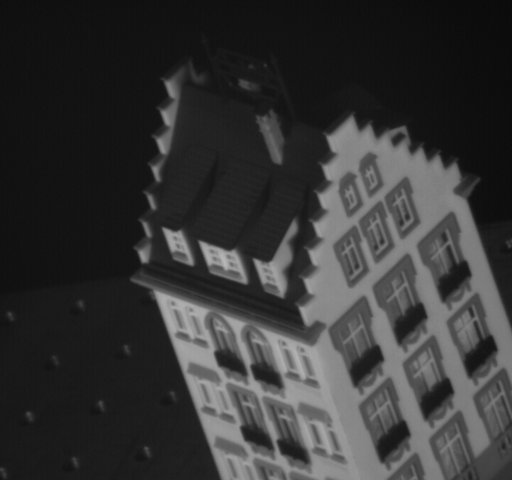
\includegraphics[width=0.14\linewidth]{./figures/video/hotel1.png} &
    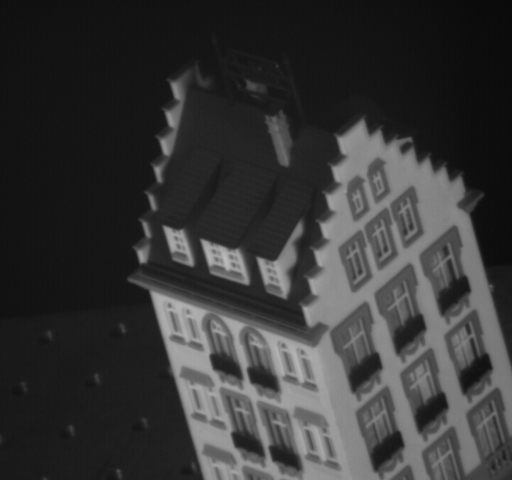
\includegraphics[width=0.14\linewidth]{./figures/video/hotel10.png} &
    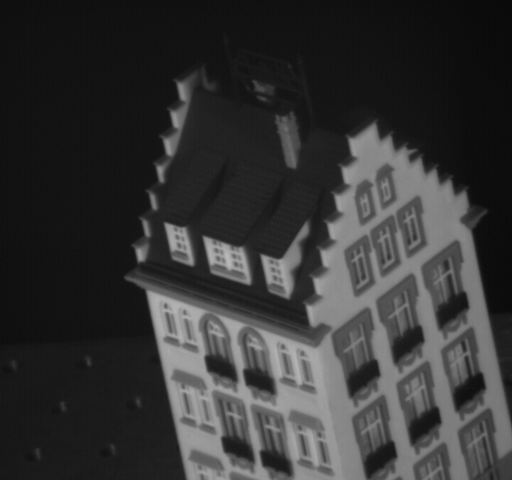
\includegraphics[width=0.14\linewidth]{./figures/video/hotel20.png} &
    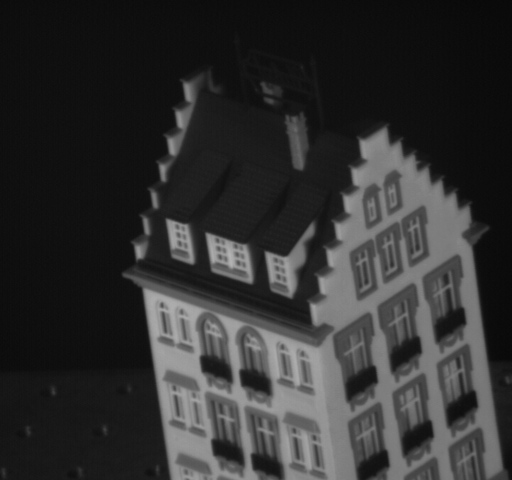
\includegraphics[width=0.14\linewidth]{./figures/video/hotel30.png} &
    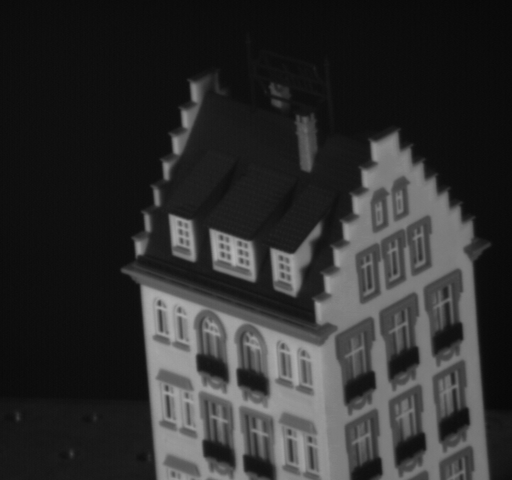
\includegraphics[width=0.14\linewidth]{./figures/video/hotel40.png} &
    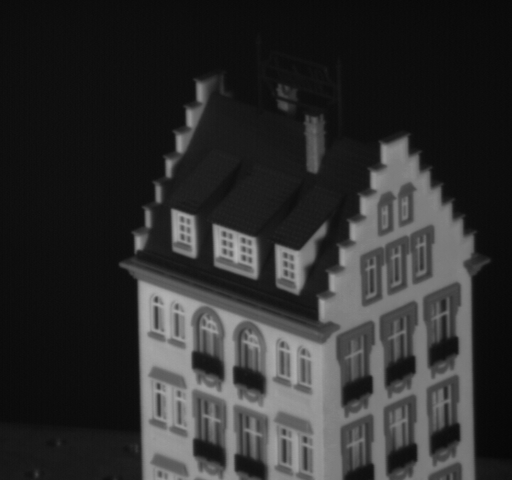
\includegraphics[width=0.14\linewidth]{./figures/video/hotel50.png}
    \end{tabular}
    \caption{Video frames.}
    \label{fig:video_frames}
\end{figure*}

\section{Keypoints Selection}
The first part of the pipeline is detecting keypoints in the first video frame. We are looking for corners as they are good for being tracked during the camera motion. The explanation comes from the fact that corners have large eigenvalues $\lambda_1$ and $\lambda_2$ as discussed in \cite{illinois_cv}. Our first attempt was to use the Harris Corner Detector with the same parameters of \cite{py_features_harris}. The results can be seen in Figure \ref{fig:harris_low} with a high number of keypoints detected. As some of the keypoints were very close together and others did not land on the target object (the hotel building), we decided to raise the threshold value to filter more of keypoints found by Harris Corner Detector. The results can be seen in Figure \ref{fig:harris_high} with many less keypoints. Although not visually apparent, some of keypoints are still clumped together. We realized that by counting the number of keypoints found which was 107 while visually it looks like we have approximately 20 keypoints.

Lastly, we decided to try OpenCV's \texttt{goodFeaturesToTrack}, which is based on \cite{good_features_paper}. In this paper, Shi et al. propose a method for feature selection  which is designed to work well for tracking under affine transformations. In other words, the \texttt{goodFeaturesToTrack} is supposed to find the keypoints that will be good for tracking throughout the video frames as opposed to Harris Corner which is only based on texturedness.

The keypoints found can be seen in Figure \ref{fig:good_features}. This final experiment seemed to produce the best results for the following reasons:
\begin{enumerate}
\item There are less keypoints clumped together;
\item All the keypoints found are on the target object (the hotel building);
\item The keypoints are well distributed around the hotel building;
\item The keypoints found are indeed corners of windows and of the roof which are good points to be tracked during the camera motion.
\end{enumerate}

\begin{figure}[ht]
  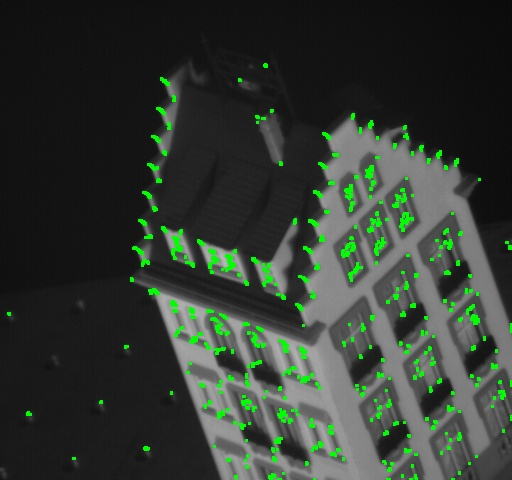
\includegraphics[width=\linewidth]{./figures/klt/harris-low-threshold.jpg}
  \caption{Keypoint selection with Harris Corner Detector (low threshold).}
  \label{fig:harris_low}
\end{figure}

\begin{figure}[ht]
  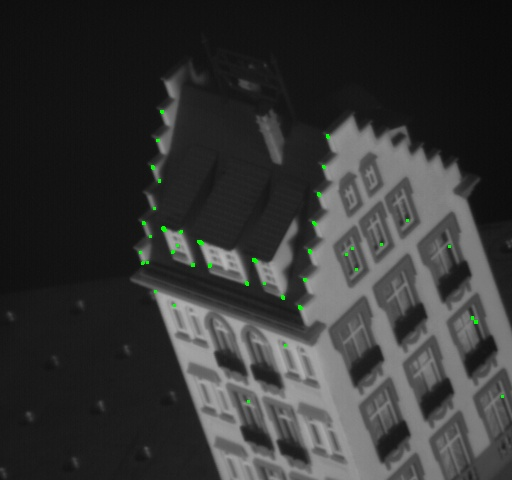
\includegraphics[width=\linewidth]{./figures/klt/harris-high-threshold.jpg}
  \caption{Keypoint selection with Harris Corner Detector (high threshold).}
  \label{fig:harris_high}
\end{figure}

\begin{figure}[ht]
  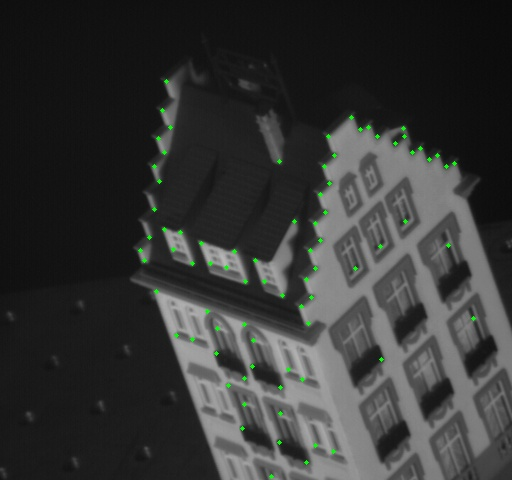
\includegraphics[width=\linewidth]{./figures/klt/good_features.jpg}
  \caption{Keypoint selection with Good Features to Track.}
  \label{fig:good_features}
\end{figure}


% Although Harris Corner Detector is able to find keypoints that seem relevant for motion tracking, the "Good Features to Track" detector is able to perform the same task but also narrow it down to 62 keypoints. As noted in \cite{py_shi_tomasi}, J. Shi and C. Tomasi published an article \cite{good_features_paper} where they made a small modification to the Harris Corner Detector showing improvements to it.
% The scoring function in Harris Corner Detector was given by:

% \[ R = \lambda_1\lambda_2 - k(\lambda_1 + \lambda _2)^2 \]

% Instead, Shi-Tomasi proposed:

% \[ R = min(\lambda_1, \lambda_2) \]


\section{Feature Tracking}
The second step of our pipeline is tracking each of the keypoints found in the previous step throughout all the video frames. For that, we have implemented the KLT algorithm.

%%%%%%%%%%%%%%%%%%%%%%%%%%%%%%
% Theory KLT
%%%%%%%%%%%%%%%%%%%%%%%%%%%%%%
\subsection{Lucas-Kanade-Tomasi (KLT)}
The Lucas-Kanade algorithm calculates the displacement of every keypoint between two consecutive video frames. Here are some key assumptions of this algorithm \cite{illinois_cv}:
\begin{itemize}
\item Brightness constancy: projection of the same point looks the same in every frame
\item Small motion: points do not move very far
\item Spatial coherence: points move like their neighbors
\end{itemize}

We can translate the first assumption into the following equality:
\begin{equation}\label{eqn:klt1}
    I(x, y, t) = I(x+u, y+v, t+1)
\end{equation}
where $u$ and $v$ describe the displacement of the pixel (x, y) at time t+1. We can then take the Taylor expansion of I (x+u, y+v, t+1) and truncate it to get to:

\begin{equation}\label{eqn:klt2}
    I(x+u, y+v, t+1) \approx I(x, y, t) + I_x \cdot u + I_y \cdot v + I_t
\end{equation}

where $I_\alpha$ represents the gradient in the dimension $\alpha$ (x, y, or t) for one pixel.
We can then move $I(x, y, t)$ to the other side of the equation:

\begin{equation}\label{eqn:klt3}
    I(x+u, y+v, t+1) - I(x, y, t) \approx I_x \cdot u + I_y \cdot v + I_t
\end{equation}

Now, given that we have equality (\ref{eqn:klt1}), we can zero the left side of the equation:

\begin{equation}\label{eqn:klt4}
    I_x \cdot u + I_y \cdot v + I_t \approx 0
\end{equation}

\begin{equation}\label{eqn:klt5}
    \begin{bmatrix}
    I_x & I_y
    \end{bmatrix}
    \cdot
    \begin{bmatrix}
    u \\ v
    \end{bmatrix}
    \approx -I_t
\end{equation}

Let's take a look at (\ref{eqn:klt5}). It has two unknown variables ($u$ and $v$) and we have only that one equation. In order to solve this linear system, we can make use of the 3rd key assumption of KLT as discussed in the beginning of this section. We can assume that within a square window of $W$ pixels, all the points will follow the same displacement. For example, if we use a window of size 5x5 pixels, we will then have 25 equations (or 25 points) to find $u$ and $v$. This linear system is written in (\ref{eqn:klt6})

\begin{equation}\label{eqn:klt6}
    \begin{bmatrix}
    I_x(p_1) & I_y(p_1) \\
    \vdots & \vdots \\
    I_x(p_N) & I_y(p_N)
    \end{bmatrix}
    \begin{bmatrix}
    u \\ v
    \end{bmatrix}
    =
    -
    \begin{bmatrix}
    I_t(p_1) \\
    \vdots \\
    I_t(p_N)
    \end{bmatrix}
\end{equation}
which can also be written as
\begin{equation}\label{eqn:klt7}
    Ad = b
\end{equation}

It is also possible to rewrite equation \ref{eqn:klt7} by multiplying both sides by $A^T$
\begin{equation}\label{eqn:klt8}
    (A^T A)d = A^T b
\end{equation}

Resolving all the matrix multiplications, we will get to (\ref{eqn:klt9}).

\begin{equation}\label{eqn:klt9}
    \begin{bmatrix}
    \sum I_x I_x & \sum I_x I_y \\
    \sum I_x I_y & \sum I_y I_y
    \end{bmatrix}
    \begin{bmatrix}
    u \\ v
    \end{bmatrix}
    =
    -
    \begin{bmatrix}
    I_t I_x \\
    I_t I_y
    \end{bmatrix}
\end{equation}

Solving this linear system will provide the translation u, v in the dimensions x, y for each keypoint.

%%%%%%%%%%%%%%%%%%%%%%%%%%%%%%
% Implementation
%%%%%%%%%%%%%%%%%%%%%%%%%%%%%%
\subsection{Implementation}
The KLT algorithm followed these steps for every pair of consecutive frames $I_1$ and $I_2$:
\begin{enumerate}
\item Apply convolution with kernel for $I_x$ defined in Table \ref{table:kernels} on $I_1$. Let's call the output $I_x$.
\item Apply convolution with kernel for $I_y$ defined in Table \ref{table:kernels} on $I_1$. Let's call the output $I_y$.
\item Apply convolution with kernel for $I_t$ defined in Table \ref{table:kernels} on $I_1$ and on $I_2$. This will output $I_{t1}$ and $I_{t2}$.
\item Calculate $I_t$ =  $I_{t2} - I_{t1}$
\item Having $I_x$, $I_y$, $I_t$, calculate the Hadamard products and then sums necessary to find the six known terms ($\sum I_x I_x$, $\sum I_x I_y$, $\sum I_x I_y$, $\sum I_y I_y$, $\sum I_x I_t$, $\sum I_y I_t$) of the system defined in (\ref{eqn:klt9}).
\item Solve the system to find $u$ and $v$ with the least squares method.
\item Discard points if the predicted coordinate is out of frame (either negative or out of the image bounds)
\end{enumerate}

% To calculate the gradient in dimensions x, y and t, we have applied convolutions on the entire image with the kernels defined in Table \ref{table:kernels}.

\begin{table}
\centering
\begin{tabular}{c c c}
$\begin{bmatrix}
    -1 & 1 \\
    -1 & 1
    \end{bmatrix}$ & $\begin{bmatrix}
    -1 & -1 \\
    1 & 1
    \end{bmatrix}$  &
    $\begin{bmatrix}
    -1 & -1 \\
    1 & 1
    \end{bmatrix}$  \\
    Kernel for $I_x$ & Kernel for $I_y$ & Kernel for $I_t$  \\
\end{tabular}
\caption{Kernels for calculating gradients}
\label{table:kernels}
\end{table}

One last detail is that our function to calculate the displacement follows a very similar interface of OpenCV's function \texttt{calcOpticalFlowPyrLK} so that we could easily replace ours by theirs during our tests. Only some of the input and output parameters were omitted as they did not make sense to our implementation.

During the development process of this algorithm, we have tried the Sobel filter as a gradient for x and y but the results were not good. The keypoints would either be always stuck on the same coordinates or they would wander around with no clear sign of being a track.

%%%%%%%%%%%%%%%%%%%%%%%%%%%%%%
% Experiments and Results
%%%%%%%%%%%%%%%%%%%%%%%%%%%%%%
\subsection{Experiments and Results}
In order to test our KLT implementation, we drew the tracks formed by each of the displacements $u$ and $v$ calculated between every consecutive video frame. This was done by simply drawing a line between point $(x,y)$ and the predicted $(x+u, y+v)$. We have also tested different window sizes (5, 15 and 30). The results for our KLT implementation can be seen in Figures \ref{fig:klt_own_w5}, \ref{fig:klt_own_w15} and \ref{fig:klt_own_w30}.
\begin{figure}[h]
  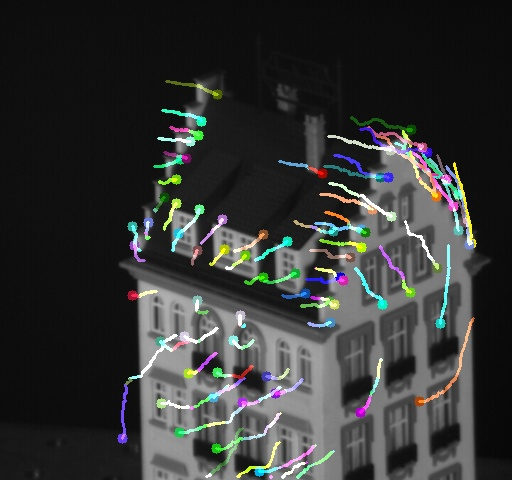
\includegraphics[width=\linewidth]{./figures/klt/klt-own-w5-hotel.jpg}
  \caption{Feature Tracking with our KLT implementation (window size 5).}
  \label{fig:klt_own_w5}
\end{figure}

\begin{figure}[h]
  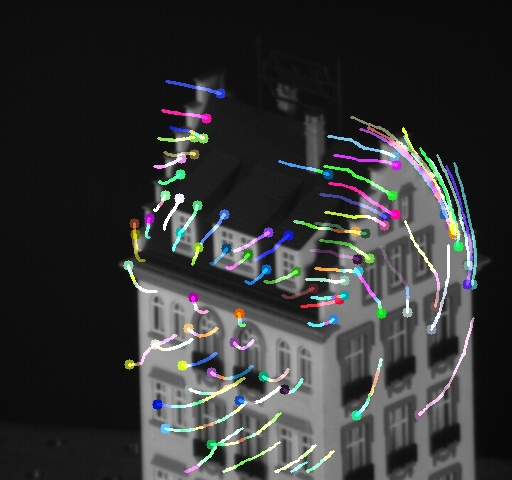
\includegraphics[width=\linewidth]{./figures/klt/klt-own-w15-hotel.jpg}
  \caption{Feature Tracking with our KLT implementation (window size 15).}
  \label{fig:klt_own_w15}
\end{figure}

\begin{figure}[h]
  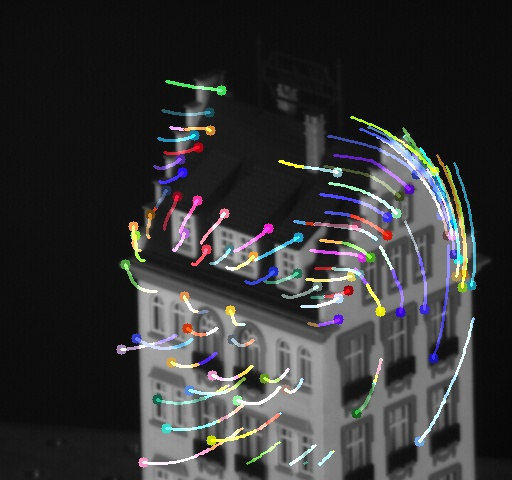
\includegraphics[width=\linewidth]{./figures/klt/klt-own-w30-hotel.jpg}
  \caption{Feature Tracking with our KLT implementation (window size 30).}
  \label{fig:klt_own_w30}
\end{figure}

\begin{figure}[h]
  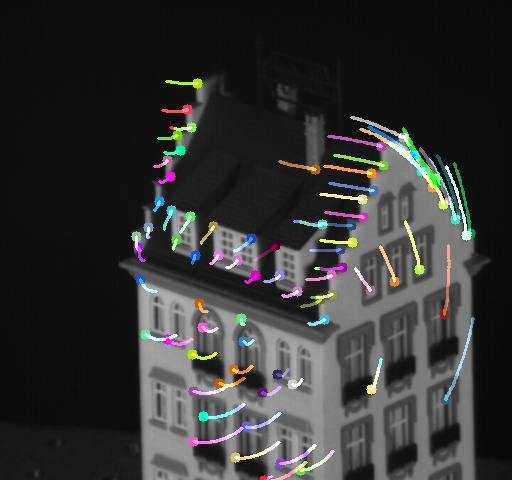
\includegraphics[width=\linewidth]{./figures/klt/klt-opencv-hotel.jpg}
  \caption{Feature Tracking with OpenCV goodFeaturesToTrack.}
  \label{fig:klt_opencv}
\end{figure}

When testing different window sizes, we noticed that a small window size of 5 creates noisy tracks whereas a larger window size of 30 creates very steady tracks. We consider that larger window sizes provide a more accurate displacement calculation. An analogy provided by \cite{illinois_cv} explains this rationale. Consider that you could see only a portion of the video frames through a square window. If that window is small, it would be hard to infer what the displacement was. Now, if the window is large, you would see more pixels moving and then you would be able to calculate the displacement with a higher accuracy. This intuition can explain in parts the phenomenon experienced with different window sizes.

For comparison and validation purposes, we have also used the tracks drawing approach but with OpenCV's \texttt{calcOpticalFlowPyrLK}. From a visual inspection, it was clear that the OpenCV's solution was very precise in keeping track of each keypoint. The results can be seen in Figure \ref{fig:klt_opencv}. We are confident to say that this could be considered a correct baseline.

Now, let us compare our implementation of KLT with OpenCV's. Overall, the tracks in our implementation obey the same direction as OpenCV's \texttt{calcOpticalFlowPyrLK}. However, we noticed that the tracks from our implementation are almost twice longer than the ones found with OpenCV. An explanation for this is that we were adding up rounding errors throughout the 50 video frames. Our system defined in (\ref{eqn:klt9}) returns $u$ and $v$ as floating point numbers and we round those values in order to find valid coordinates (which have to be integers). Moreover, it was expected that we would have different results as OpenCV uses a more robust algorithm which applies the Lucas-Kanade algorithm on different levels of a pyramid.


% THIS WAS an attempt to put all 4 images of KLT into one table but it wasn't good as it would probably use an entire page of its own.
% \begin{figure*}[tb]
% \centering
% \begin{subfigure}{0.45\textwidth}
% 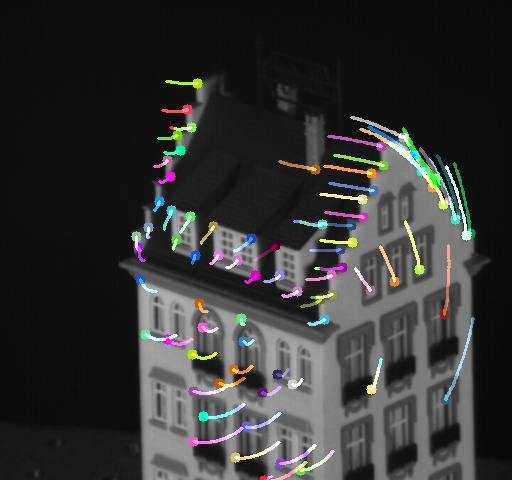
\includegraphics[width=0.9\linewidth]{./figures/klt/klt-opencv-hotel.jpg}
% \caption{Using OpenCV goodFeaturesToTrack}
% \label{fig:subim1}
% \end{subfigure}
% \begin{subfigure}{0.45\textwidth}
% 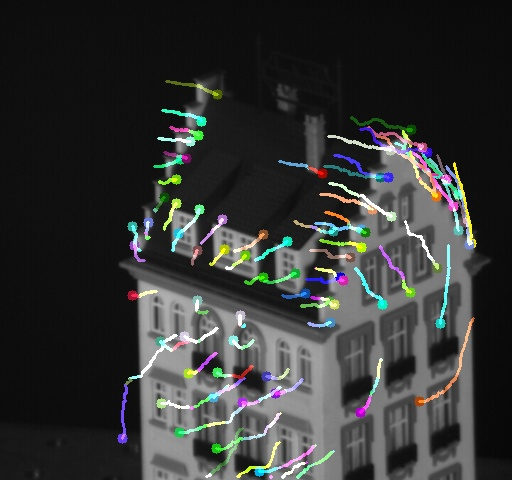
\includegraphics[width=0.9\linewidth]{./figures/klt/klt-own-w5-hotel.jpg}
% \caption{Own KLT implementation (window size 5)}
% \label{fig:subim2}
% \end{subfigure}
% \hfill
% \begin{subfigure}{0.45\textwidth}
% 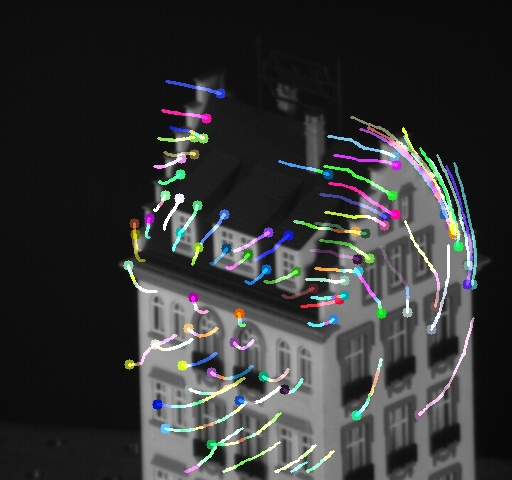
\includegraphics[width=0.9\linewidth]{./figures/klt/klt-own-w15-hotel.jpg}
% \caption{Own KLT implementation (window size 15)}
% \label{fig:subim3}
% \end{subfigure}
% \begin{subfigure}{0.45\textwidth}
% 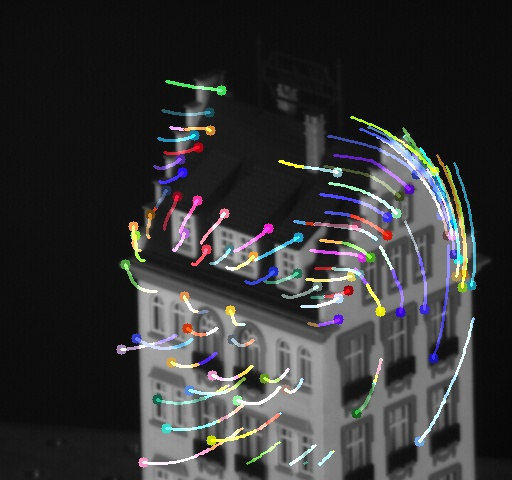
\includegraphics[width=0.9\linewidth]{./figures/klt/klt-own-w30-hotel.jpg}
% \caption{Own KLT implementation (window size 30)}
% \label{fig:subim4}
% \end{subfigure}
% \caption{Feature Tracking Results}
% \label{fig:klt_results}
% \end{figure*}

% \begin{figure*}[tb]
%     \centering
%     \begin{tabular}{c c }

% \begin{figure}[ht]

%   \caption{Feature Tracking with OpenCV calcOpticalFlowPyrLK.}
%   \label{fig:klt_hotel_opencv}
% \end{figure}
% &

% 4 images of KLT results

\section{Structure from Motion}
In this work we implemented the factorization method, which can robustly recover shape and motion from a sequence of images under orthographic projection. In the factorization method, an image is represented as a measurement matrix $\bm{W}^{2F \times P}$, which is made up of the horizontal and vertical coordinates of $P$ points tracked through $F$ frames. The following steps are based on \cite{morita}.

The measurement matrix can be factored into the product of two matrices $\bm{M}^{2F \times 3}$ and $\bm{S}^{3 \times P}$. Here, $\bm{M}$ is a matrix that represents camera rotation, and $\bm{S}$ is a matrix that represents shape in a coordinate system attached to the object centroid.

Suppose that the camera orientation at frame $f$ is represented by orthonormal vectors $i_f$ , $j_f$ , and $k_f$ , where $i_f$ corresponds to the $x$-axis of the image plane, and $j_f$ to the $y$-axis. The vectors $i_f$ and $j_f$ are collected over $F$ frames into a motion matrix $\bm{M}$ such that
\[
\bm{M} =
\begin{bmatrix}
    i_{1}^T \\
    \vdots \\
    i_{F}^T \\
    j_{1}^T \\
    \vdots \\
    j_{F}^T \\
\end{bmatrix}
\]
Let $s_p$ be the location of feature $p$ in a fixed world coordinate system, whose origin is set at the center-of-mass of all the feature points. These vectors are then collected into a shape matrix $\bm{S}$ such that
\[
\bm{S} =
\begin{bmatrix}
    s_1, \dots, s_p
\end{bmatrix}
\]

The actual procedure of the factorization method consists of two steps. First, the measurement matrix is factorized into two matrices of rank three using the singular value decomposition: $\bm{W} = \bm{U}\bm{\Sigma}\bm{V}^T$.

By setting $\hat{\bm{M}} = \bm{U}$ and $\hat{\bm{S}} = \bm{\Sigma V^T}$ we can factorize $\bm{W}$ into $\hat{\bm{M}}\hat{\bm{S}}$. This decomposition is not completely unique: It is unique only up to an affine transformation. The second step of the method is necessary to find a non-singular matrix $\bm{A}^{3 \times 3}$, which transforms $\hat{\bm{M}}$ and $\hat{\bm{S}}$ into the true solutions $\bm{M}$ and $\bm{S}$ as follows.
\begin{align*}
    \bm{M} &= \hat{\bm{M}}\bm{A}\\
    \bm{S} &= \bm{A}^{-1}\hat{\bm{S}}
\end{align*}

Observing that rows $i_f$ and $j_f$ of $\bm{M}$ must satisfy the normalization constraints $i_{f}^Ti_{f} = j_{f}^Tj_{f} = 1$ and $i_{f}^Tj_{f} = 0$. We obtain the system of 3F over-determined equations, such that
\begin{align}
    \hat{i}_{f}^T\bm{L}\hat{i}_{f} &= 1 \nonumber \\
    \hat{j}_{f}^T\bm{L}\hat{j}_{f} &= 1 \nonumber \\
    \hat{i}_{f}^T\bm{L}\hat{j}_{f} &= 0
    \label{eqn:system}
\end{align}

\begin{figure*}[tb]
    \centering
    \begin{tabular}{c c c c}
    \rotatebox{90}{Our implementation} & 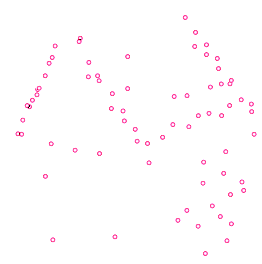
\includegraphics[width=0.3\linewidth]{./figures/3d/our/snapshot01.png} &
    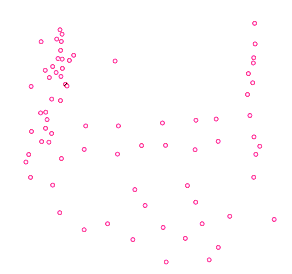
\includegraphics[width=0.3\linewidth]{./figures/3d/our/snapshot03.png} &
    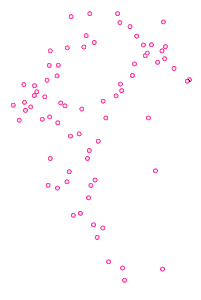
\includegraphics[width=0.22\linewidth]{./figures/3d/our/snapshot04.png}\\
    \rotatebox{90}{OpenCV's implementation} &
    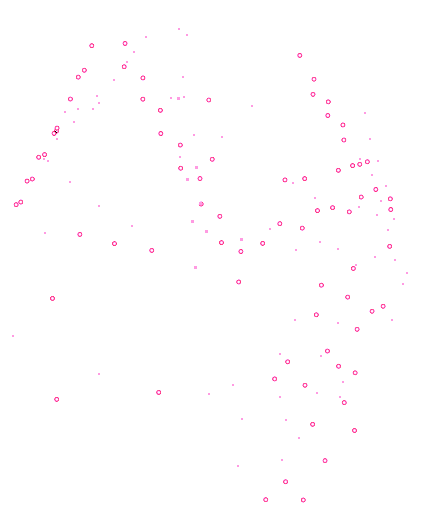
\includegraphics[width=0.25\linewidth]{./figures/3d/cv/snapshot00.png} &
    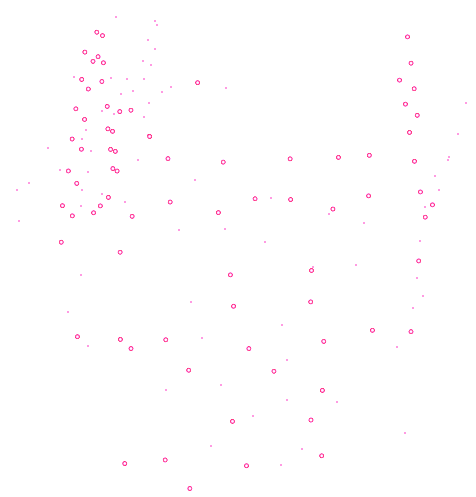
\includegraphics[width=0.3\linewidth]{./figures/3d/cv/snapshot01.png} &
    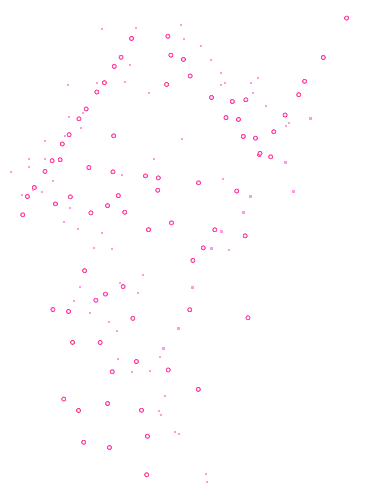
\includegraphics[width=0.22\linewidth]{./figures/3d/cv/snapshot02.png}\\
    & a.~Hotel view from one side. & b.~Hotel view from front. & c.~ Hotel view from the other side.\\
    \end{tabular}
    \caption{$3D$ points of the hotel building.}
    \label{fig:3dcloud}
\end{figure*}

Where $\bm{L}^{3 \times 3}$ is a symmetric matrix $\bm{L} = \bm{A}\bm{A}^T$ built with vector $\bm{l}$, which can be found with Least Squares. And $\hat{i}_{f}$ and $\hat{j}_{f}$ are rows of $\hat{\bm{M}}$. The system in Eq. \ref{eqn:system} can be rewritten as $\bm{G}^{3F \times 6}\bm{l}^6 = \bm{c}^{3F}$. $\bm{G}$ is defined as
\[
\bm{G} =
\begin{bmatrix}
    g^T(i_{1},i_{1}) \\
    \vdots \\
    g^T(i_{F},i_{F}) \\
    g^T(j_{1},j_{1}) \\
    \vdots \\
    g^T(j_{F},j_{F}) \\
    g^T(i_{1},j_{1}) \\
    \vdots \\
    g^T(j_{F},j_{F}) \\
\end{bmatrix}
\]
and $g^T(a_{f},b_{f}) = a_{f1}b_{f1}\quad a_{f1}b_{f2} + a_{f2}b_{f1}\quad a_{f1}b_{f3} + a_{f3}b_{f1}\quad a_{f2}b_{f2}\quad a_{f2}b_{f3} + a_{f3}b_{f2}\quad a_{f3}b_{f3}$.

The simplest solution of the system is given by the pseudo-inverse method, such that $\bm{l} = (\bm{G}^T\bm{G})^{-1}\bm{G}^T\bm{c}$. In order to eliminate the affine ambiguity, we compute the Cholesky decomposition of $\bm{L} = \bm{A}\bm{A}^T$ to recover $\bm{A}$.

The matrix $\bm{A}$ is an affine transform which transforms $\hat{\bm{M}}$ into $\bm{M}$ in the motion space, while the matrix $\bm{A}^{-1}$ transforms $\hat{\bm{S}}$ into $\bm{S}$ in the shape space. Obtaining this transform is the main purpose of the second step of the factorization method, which we call metric transformation.

Figure \ref{fig:3dcloud} illustrates the $3D$ cloud points representation of the frames with both our approach and OpenCV's. Comparing the figures we can see that our results are close to those yielded by OpenCV.

One side of the hotel (Figure \ref{fig:3dcloud}a) is more distinguishable than the other (Figure \ref{fig:3dcloud}c) in our implementation comparing with OpenCV, this is because erros are introduced in our KLT implementation decrease the quality of the reconstruction.

The front (Figure \ref{fig:3dcloud}b) follows the same reasoning: points too spread in the space in such way that difficult the identification of the Hotel. Meanwhile OpenCV's the points have a more structured behavior.

\section{Conclusion}
The task of this project was to reconstruct the 3D shape of a target object using a series of video frames. We split this task in three sub-tasks: keypoint selection, feature tracking, and structure from motion. To select the keypoints, we used OpenCV's implementation of the Shi-Tomasi Corner Detector (\texttt{goodFeaturesToTrack}), which gave better results than the Harris Corner Detector.

For the tracking of features, we implemented the Lucas-Kanade-Tomasi algorithm to compute the optical flow in the video frames. The results were reasonably good, especially considering that this implementation does not use pyramids.

Finally, we implemented the factorization method by Tomasi and Kanade for the structure from motion sub-task. Again, good results were obtained - we could reconstruct successfully the shape of the hotel building using the available 50 video frames. The output is generated in the Polygon File Format (PLY), and can be viewed in an application like MeshLab.

\begin{thebibliography}{00}
    \bibitem{good_features_paper} J. Shi and C. Tomasi (1994, June). ``Good features to track.'' In 1994 Proceedings of IEEE Conference on Computer Vision and Pattern Recognition.
    \bibitem{tomasi_kanade} C. Tomasi and T. Kanade, ``Detection and tracking of feature points.'' Tech. Rep., Carnegie Mellon University
    \bibitem{lucas_kanade} B.D. Lucas, T. Kanade, et al., ``An iterative image registration technique with an application to stereo vision,'' 1981.
    \bibitem{sfm_paper} C. Tomasi and T. Kanade, ``Shape and motion from image streams under orthography: A factorization method,'' International Journal of Computer Vision, vol. 9, no. 2, pp. 137–154, 1992.

    \bibitem{py_features_harris} Site visited on October 14, 2018, from \url{https://docs.opencv.org/3.0-beta/doc/py_tutorials/py_feature2d/py_features_harris/py_features_harris.html}
    \bibitem{py_shi_tomasi} Site visited on October 14, 2018, from \url{https://docs.opencv.org/3.0-beta/doc/py_tutorials/py_feature2d/py_shi_tomasi/py_shi_tomasi.html}
    \bibitem{opencv_klt} Site visited on October 14, 2018, from \url{https://docs.opencv.org/3.3.1/d7/d8b/tutorial_py_lucas_kanade.html}
    \bibitem{brown_cv} CS 143: Introduction to Computer Vision. Site visited on October 14, 2018, from \url{http://cs.brown.edu/courses/cs143/2011/proj5/}
    \bibitem{illinois_cv} University of Illinois. Computer Vision. Site visited on October 14, 2018, from \url{https://courses.engr.illinois.edu/cs543/sp2012/lectures/Lecture%2008%20-%20Feature%20Tracking%20and%20Optical%20Flow%20-%20Vision_Spring2012.pdf}
    \bibitem{morita} Morita, T., \& Kanade, T. (1997). ``A sequential factorization method for recovering shape and motion from image streams.'' IEEE Transactions on Pattern Analysis \& Machine Intelligence, (8), 858-867.


\end{thebibliography}
\end{document}
